% Options for packages loaded elsewhere
\PassOptionsToPackage{unicode}{hyperref}
\PassOptionsToPackage{hyphens}{url}
%
\documentclass[
]{article}
\usepackage{amsmath,amssymb}
\usepackage{lmodern}
\usepackage{iftex}
\ifPDFTeX
  \usepackage[T1]{fontenc}
  \usepackage[utf8]{inputenc}
  \usepackage{textcomp} % provide euro and other symbols
\else % if luatex or xetex
  \usepackage{unicode-math}
  \defaultfontfeatures{Scale=MatchLowercase}
  \defaultfontfeatures[\rmfamily]{Ligatures=TeX,Scale=1}
  \setmainfont[]{SourceSansPro}
\fi
% Use upquote if available, for straight quotes in verbatim environments
\IfFileExists{upquote.sty}{\usepackage{upquote}}{}
\IfFileExists{microtype.sty}{% use microtype if available
  \usepackage[]{microtype}
  \UseMicrotypeSet[protrusion]{basicmath} % disable protrusion for tt fonts
}{}
\makeatletter
\@ifundefined{KOMAClassName}{% if non-KOMA class
  \IfFileExists{parskip.sty}{%
    \usepackage{parskip}
  }{% else
    \setlength{\parindent}{0pt}
    \setlength{\parskip}{6pt plus 2pt minus 1pt}}
}{% if KOMA class
  \KOMAoptions{parskip=half}}
\makeatother
\usepackage{xcolor}
\usepackage[margin=1in]{geometry}
\usepackage{longtable,booktabs,array}
\usepackage{calc} % for calculating minipage widths
% Correct order of tables after \paragraph or \subparagraph
\usepackage{etoolbox}
\makeatletter
\patchcmd\longtable{\par}{\if@noskipsec\mbox{}\fi\par}{}{}
\makeatother
% Allow footnotes in longtable head/foot
\IfFileExists{footnotehyper.sty}{\usepackage{footnotehyper}}{\usepackage{footnote}}
\makesavenoteenv{longtable}
\usepackage{graphicx}
\makeatletter
\def\maxwidth{\ifdim\Gin@nat@width>\linewidth\linewidth\else\Gin@nat@width\fi}
\def\maxheight{\ifdim\Gin@nat@height>\textheight\textheight\else\Gin@nat@height\fi}
\makeatother
% Scale images if necessary, so that they will not overflow the page
% margins by default, and it is still possible to overwrite the defaults
% using explicit options in \includegraphics[width, height, ...]{}
\setkeys{Gin}{width=\maxwidth,height=\maxheight,keepaspectratio}
% Set default figure placement to htbp
\makeatletter
\def\fps@figure{htbp}
\makeatother
\setlength{\emergencystretch}{3em} % prevent overfull lines
\providecommand{\tightlist}{%
  \setlength{\itemsep}{0pt}\setlength{\parskip}{0pt}}
\setcounter{secnumdepth}{-\maxdimen} % remove section numbering
\ifLuaTeX
  \usepackage{selnolig}  % disable illegal ligatures
\fi
\IfFileExists{bookmark.sty}{\usepackage{bookmark}}{\usepackage{hyperref}}
\IfFileExists{xurl.sty}{\usepackage{xurl}}{} % add URL line breaks if available
\urlstyle{same} % disable monospaced font for URLs
\hypersetup{
  pdftitle={Практическая работа №5. Линейная регрессия. Оценка адекватности модели, оценка доверительных интервалов параметров.},
  pdfauthor={Юрченков Иван Александрович, ассистент кафедры ПМ},
  hidelinks,
  pdfcreator={LaTeX via pandoc}}

\title{Практическая работа №5. Линейная регрессия. Оценка адекватности
модели, оценка доверительных интервалов параметров.}
\author{Юрченков Иван Александрович, ассистент кафедры ПМ}
\date{2022-10-17}

\begin{document}
\maketitle

\begin{verbatim}
## 
## Присоединяю пакет: 'dplyr'
\end{verbatim}

\begin{verbatim}
## Следующие объекты скрыты от 'package:stats':
## 
##     filter, lag
\end{verbatim}

\begin{verbatim}
## Следующие объекты скрыты от 'package:base':
## 
##     intersect, setdiff, setequal, union
\end{verbatim}

\hypertarget{ux43fux43eux441ux442ux430ux43dux43eux432ux43aux430-ux437ux430ux434ux430ux447ux438-ux434ux43bux44f-ux432ux44bux43fux43eux43bux43dux435ux43dux438ux44f-ux43fux440ux430ux43aux442ux438ux447ux435ux441ux43aux43eux439-ux440ux430ux431ux43eux442ux44b}{%
\section{\texorpdfstring{\textbf{Постановка задачи для выполнения
практической
работы}}{Постановка задачи для выполнения практической работы}}\label{ux43fux43eux441ux442ux430ux43dux43eux432ux43aux430-ux437ux430ux434ux430ux447ux438-ux434ux43bux44f-ux432ux44bux43fux43eux43bux43dux435ux43dux438ux44f-ux43fux440ux430ux43aux442ux438ux447ux435ux441ux43aux43eux439-ux440ux430ux431ux43eux442ux44b}}

Для выполнения практического задания необходимо:

\begin{enumerate}
\def\labelenumi{\arabic{enumi}.}
\item
  Открыть папку, соотвествующую своей группе.
\item
  Открыть папку с вариантом, совпадающим с вашим номером в списке.
\end{enumerate}

В папке 3 файла с данными.

\begin{enumerate}
\def\labelenumi{\arabic{enumi}.}
\tightlist
\item
  1-ый файл содержит 2 ряда данных. Первый стоблец \(\ x\ \) содержит
  факторную переменную, второй столбец \(\ y\ \) результирующую. Для
  первого файла необходимо:
\end{enumerate}

\begin{itemize}
\item
  Оценить коэффициент корреляции Пирсона \(\ r(x, y)\ \) между двумя
  переменными в первом и втором столбце.
\item
  По шкале Чеддока оценить хакактеристику корреляционной связи между
  величинами.
\item
  Проверить статистическую значимость коэффициента корреляции Пирсона с
  помощью \(t\)-статистики.
\item
  Построить доверительный интервал для \(\ r(x, y)\ \) с надежностью
  \(\ \gamma\ = \ 0.95\).
\item
  Построить линейную регрессию между столбцами, оценить значение
  коэффициентов линейной зависимости.
\item
  Оценить значимость полученных коэффициентов прямой.
\item
  Построить доверительные интервалы для полученных коэффициентов.
\item
  Оценить адекватность модели \emph{по коэффициенту детерминации}.
\item
  Оценить интервал прогноза для линейной модели на \$ft = 3\$ значения
  вперед.
\end{itemize}

\begin{enumerate}
\def\labelenumi{\arabic{enumi}.}
\setcounter{enumi}{1}
\tightlist
\item
  2-ой файл содержит 4 ряда данных. Первый ряд (столбец) содержит
  количественную факторную переменную, следующие два - качественную
  факторную переменную, последний - результирующую переменную. Для
  второго файла данных необходимо:
\end{enumerate}

\begin{itemize}
\item
  Необходимо с помощью теста Чоу обосновать необходимость деления
  выборки по одной из качественных факторных переменных.
\item
  Произвести разбиение и построить две линейных регрессии, оценить
  коэффициенты моделей.
\end{itemize}

\begin{enumerate}
\def\labelenumi{\arabic{enumi}.}
\setcounter{enumi}{2}
\tightlist
\item
  3-ий файл содержит 2 ряда данных. Для третьего файла данных
  необходимо:
\end{enumerate}

\begin{itemize}
\item
  Необходимо двумя способами (тест Спирмена и тест Гольдфельда-Квандта)
  определить, присутствует ли в данных гетероскедастичность.
\item
  Построить линейную регрессию, оценить значения коэффициентов модели.
\item
  Оценить значимость полученных коэффициентов и адекватность модели.
\item
  Все расчеты проводить для уровня значимости \(\alpha = 0.05\).
\end{itemize}

\hypertarget{ux43fux440ux438ux43cux435ux440-ux43fux440ux43eux432ux435ux434ux435ux43dux438ux44f-ux440ux435ux433ux440ux435ux441ux441ux438ux43eux43dux43dux43eux433ux43e-ux430ux43dux430ux43bux438ux437ux430-ux434ux43bux44f-ux440ux44fux434ux430-ux434ux430ux43dux43dux44bux445}{%
\section{\texorpdfstring{\textbf{Пример проведения регрессионного
анализа для ряда
данных}}{Пример проведения регрессионного анализа для ряда данных}}\label{ux43fux440ux438ux43cux435ux440-ux43fux440ux43eux432ux435ux434ux435ux43dux438ux44f-ux440ux435ux433ux440ux435ux441ux441ux438ux43eux43dux43dux43eux433ux43e-ux430ux43dux430ux43bux438ux437ux430-ux434ux43bux44f-ux440ux44fux434ux430-ux434ux430ux43dux43dux44bux445}}

\hypertarget{ux438ux441ux441ux43bux435ux434ux443ux435ux43cux44bux439-ux440ux44fux434-ux434ux430ux43dux43dux44bux445}{%
\subsection{\texorpdfstring{\textbf{Исследуемый ряд
данных}}{Исследуемый ряд данных}}\label{ux438ux441ux441ux43bux435ux434ux443ux435ux43cux44bux439-ux440ux44fux434-ux434ux430ux43dux43dux44bux445}}

Для демонстрации проведения регрессионного анализа над рядом данных
выбран набор данных цен на алмазы (diamonds), являющийся классическим
набором данных для проверки регрессионных моделей и алгоритмов
идентификации, очистки или корректировки выбросов. Всего в наборе данных
10 переменных. В рассмотрение возьмем только две из них:

\begin{enumerate}
\def\labelenumi{\arabic{enumi}.}
\item
  carat \(-\) караты алмазов,
\item
  price \(-\) цена алмазов.
\end{enumerate}

Предварительный анализ данных рядов показывает их нелинейную
зависимость, похожую на параболическую, и чтобы избежать её в линейном
регрессионном анализе, принято решение \textbf{прологарифмировать} оба
ряда данных для спрямления зависимости в декартовых координатах.

Рассмотрим таблицу переменных парных данных
\(\left(ln(x), ln(y)\right)\) одинаковой длины без пропущенных значений
для данных о цене алмазов (\(y\)) с категориальными параметрами:
\(cut = Ideal\) (огранка), \(color = J\) (цвет), \(clarity = SI2\)
(чистота).

\begin{longtable}[]{@{}
  >{\raggedright\arraybackslash}p{(\columnwidth - 22\tabcolsep) * \real{0.0714}}
  >{\raggedright\arraybackslash}p{(\columnwidth - 22\tabcolsep) * \real{0.1143}}
  >{\raggedright\arraybackslash}p{(\columnwidth - 22\tabcolsep) * \real{0.0857}}
  >{\raggedright\arraybackslash}p{(\columnwidth - 22\tabcolsep) * \real{0.0571}}
  >{\raggedright\arraybackslash}p{(\columnwidth - 22\tabcolsep) * \real{0.1000}}
  >{\raggedright\arraybackslash}p{(\columnwidth - 22\tabcolsep) * \real{0.0857}}
  >{\raggedright\arraybackslash}p{(\columnwidth - 22\tabcolsep) * \real{0.0571}}
  >{\raggedright\arraybackslash}p{(\columnwidth - 22\tabcolsep) * \real{0.1000}}
  >{\raggedright\arraybackslash}p{(\columnwidth - 22\tabcolsep) * \real{0.0857}}
  >{\raggedright\arraybackslash}p{(\columnwidth - 22\tabcolsep) * \real{0.0571}}
  >{\raggedright\arraybackslash}p{(\columnwidth - 22\tabcolsep) * \real{0.1000}}
  >{\raggedright\arraybackslash}p{(\columnwidth - 22\tabcolsep) * \real{0.0857}}@{}}
\caption{Таблица данных}\tabularnewline
\toprule()
\begin{minipage}[b]{\linewidth}\raggedright
\textbf{n}
\end{minipage} & \begin{minipage}[b]{\linewidth}\raggedright
ln(x)
\end{minipage} & \begin{minipage}[b]{\linewidth}\raggedright
ln(y)
\end{minipage} & \begin{minipage}[b]{\linewidth}\raggedright
n
\end{minipage} & \begin{minipage}[b]{\linewidth}\raggedright
ln(x)
\end{minipage} & \begin{minipage}[b]{\linewidth}\raggedright
ln(y)
\end{minipage} & \begin{minipage}[b]{\linewidth}\raggedright
n
\end{minipage} & \begin{minipage}[b]{\linewidth}\raggedright
ln(x)
\end{minipage} & \begin{minipage}[b]{\linewidth}\raggedright
ln(y)
\end{minipage} & \begin{minipage}[b]{\linewidth}\raggedright
n
\end{minipage} & \begin{minipage}[b]{\linewidth}\raggedright
ln(x)
\end{minipage} & \begin{minipage}[b]{\linewidth}\raggedright
ln(y)
\end{minipage} \\
\midrule()
\endfirsthead
\toprule()
\begin{minipage}[b]{\linewidth}\raggedright
\textbf{n}
\end{minipage} & \begin{minipage}[b]{\linewidth}\raggedright
ln(x)
\end{minipage} & \begin{minipage}[b]{\linewidth}\raggedright
ln(y)
\end{minipage} & \begin{minipage}[b]{\linewidth}\raggedright
n
\end{minipage} & \begin{minipage}[b]{\linewidth}\raggedright
ln(x)
\end{minipage} & \begin{minipage}[b]{\linewidth}\raggedright
ln(y)
\end{minipage} & \begin{minipage}[b]{\linewidth}\raggedright
n
\end{minipage} & \begin{minipage}[b]{\linewidth}\raggedright
ln(x)
\end{minipage} & \begin{minipage}[b]{\linewidth}\raggedright
ln(y)
\end{minipage} & \begin{minipage}[b]{\linewidth}\raggedright
n
\end{minipage} & \begin{minipage}[b]{\linewidth}\raggedright
ln(x)
\end{minipage} & \begin{minipage}[b]{\linewidth}\raggedright
ln(y)
\end{minipage} \\
\midrule()
\endhead
\textbf{1} & -1.171 & 5.841 & \textbf{31} & 0.095 & 8.439 & \textbf{61}
& 0.571 & 8.958 & \textbf{91} & -1.109 & 5.903 \\
\textbf{2} & 0.020 & 7.965 & \textbf{32} & 0.231 & 8.446 & \textbf{62} &
0.531 & 9.048 & \textbf{92} & -0.892 & 6.594 \\
\textbf{3} & 0.000 & 8.150 & \textbf{33} & 0.182 & 8.447 & \textbf{63} &
0.698 & 9.307 & \textbf{93} & -0.942 & 6.111 \\
\textbf{4} & 0.000 & 8.168 & \textbf{34} & 0.215 & 8.448 & \textbf{64} &
0.723 & 9.327 & \textbf{94} & -0.635 & 6.752 \\
\textbf{5} & 0.077 & 8.171 & \textbf{35} & 0.199 & 8.450 & \textbf{65} &
0.703 & 9.334 & \textbf{95} & -0.673 & 6.786 \\
\textbf{6} & 0.049 & 8.193 & \textbf{36} & 0.239 & 8.454 & \textbf{66} &
0.723 & 9.336 & \textbf{96} & -0.654 & 6.829 \\
\textbf{7} & 0.010 & 8.225 & \textbf{37} & 0.231 & 8.464 & \textbf{67} &
0.708 & 9.389 & \textbf{97} & -0.616 & 6.886 \\
\textbf{8} & 0.039 & 8.223 & \textbf{38} & 0.182 & 8.465 & \textbf{68} &
0.732 & 9.407 & \textbf{98} & -0.635 & 6.910 \\
\textbf{9} & 0.010 & 8.243 & \textbf{39} & 0.182 & 8.465 & \textbf{69} &
0.698 & 9.439 & \textbf{99} & -0.462 & 6.971 \\
\textbf{10} & 0.058 & 8.227 & \textbf{40} & 0.239 & 8.472 & \textbf{70}
& 0.718 & 9.446 & \textbf{100} & -0.357 & 7.477 \\
\textbf{11} & 0.010 & 8.290 & \textbf{41} & 0.215 & 8.473 & \textbf{71}
& 0.708 & 9.451 & \textbf{101} & -0.357 & 7.510 \\
\textbf{12} & 0.010 & 8.293 & \textbf{42} & 0.231 & 8.489 & \textbf{72}
& 0.703 & 9.452 & \textbf{102} & -0.357 & 7.513 \\
\textbf{13} & 0.030 & 8.296 & \textbf{43} & 0.239 & 8.503 & \textbf{73}
& 0.728 & 9.455 & \textbf{103} & -0.274 & 7.514 \\
\textbf{14} & 0.030 & 8.307 & \textbf{44} & 0.239 & 8.521 & \textbf{74}
& 0.698 & 9.458 & \textbf{104} & -0.342 & 7.550 \\
\textbf{15} & 0.104 & 8.312 & \textbf{45} & 0.086 & 8.524 & \textbf{75}
& 0.829 & 9.488 & \textbf{105} & -0.329 & 7.563 \\
\textbf{16} & 0.104 & 8.317 & \textbf{46} & 0.207 & 8.534 & \textbf{76}
& 0.698 & 9.492 & \textbf{106} & -0.288 & 7.573 \\
\textbf{17} & 0.010 & 8.318 & \textbf{47} & 0.207 & 8.548 & \textbf{77}
& 0.798 & 9.525 & \textbf{107} & -0.357 & 7.624 \\
\textbf{18} & 0.104 & 8.319 & \textbf{48} & 0.293 & 8.570 & \textbf{78}
& 0.829 & 9.527 & \textbf{108} & -0.211 & 7.650 \\
\textbf{19} & 0.049 & 8.325 & \textbf{49} & 0.293 & 8.586 & \textbf{79}
& 0.829 & 9.582 & \textbf{109} & 0.020 & 7.867 \\
\textbf{20} & 0.095 & 8.333 & \textbf{50} & 0.322 & 8.660 & \textbf{80}
& 0.916 & 9.582 & \textbf{110} & 0.000 & 7.885 \\
\textbf{21} & 0.010 & 8.337 & \textbf{51} & 0.445 & 8.660 & \textbf{81}
& 0.916 & 9.632 & & & \\
\textbf{22} & 0.131 & 8.346 & \textbf{52} & 0.322 & 8.694 & \textbf{82}
& 0.904 & 9.644 & & & \\
\textbf{23} & 0.095 & 8.349 & \textbf{53} & 0.419 & 8.714 & \textbf{83}
& 0.916 & 9.680 & & & \\
\textbf{24} & 0.113 & 8.372 & \textbf{54} & 0.315 & 8.715 & \textbf{84}
& 0.928 & 9.680 & & & \\
\textbf{25} & 0.030 & 8.377 & \textbf{55} & 0.507 & 8.760 & \textbf{85}
& 1.102 & 9.683 & & & \\
\textbf{26} & 0.049 & 8.381 & \textbf{56} & 0.438 & 8.825 & \textbf{86}
& 0.900 & 9.709 & & & \\
\textbf{27} & 0.122 & 8.383 & \textbf{57} & 0.438 & 8.849 & \textbf{87}
& 0.967 & 9.736 & & & \\
\textbf{28} & 0.174 & 8.414 & \textbf{58} & 0.464 & 8.876 & \textbf{88}
& 0.959 & 9.753 & & & \\
\textbf{29} & 0.182 & 8.414 & \textbf{59} & 0.531 & 8.918 & \textbf{89}
& 1.001 & 9.787 & & & \\
\textbf{30} & 0.182 & 8.416 & \textbf{60} & 0.536 & 8.948 & \textbf{90}
& 0.956 & 9.818 & & & \\
\bottomrule()
\end{longtable}

Далее наши логарифмированные данные обозначим как
\(x := ln(x), \quad y := ln(y),\) и примем данные переменные как
рассматриваемые в нашем регрессионном анализе факторные и результирующие
соответственно.

В рассматриваемой таблице данных присутствует \(n = 110\) наблюдений для
каждой из рассматриваемых переменных.

Построим гистограммы распределений наших данных в каждой из переменных:

\(\ \)

\begin{verbatim}
##        groupnames abs_freq   rel_freq    low   high     med     h
## 1  (-1.17,-0.846]        4 0.03636364 -1.170 -0.846 -1.0080 0.324
## 2 (-0.846,-0.522]        5 0.04545455 -0.846 -0.522 -0.6840 0.324
## 3 (-0.522,-0.197]       10 0.09090909 -0.522 -0.197 -0.3595 0.325
## 4  (-0.197,0.128]       29 0.26363636 -0.197  0.128 -0.0345 0.325
## 5   (0.128,0.453]       28 0.25454545  0.128  0.453  0.2905 0.325
## 6   (0.453,0.777]       19 0.17272727  0.453  0.777  0.6150 0.324
## 7     (0.777,1.1]       15 0.13636364  0.777  1.100  0.9385 0.323
\end{verbatim}

\(\ \)

\begin{center}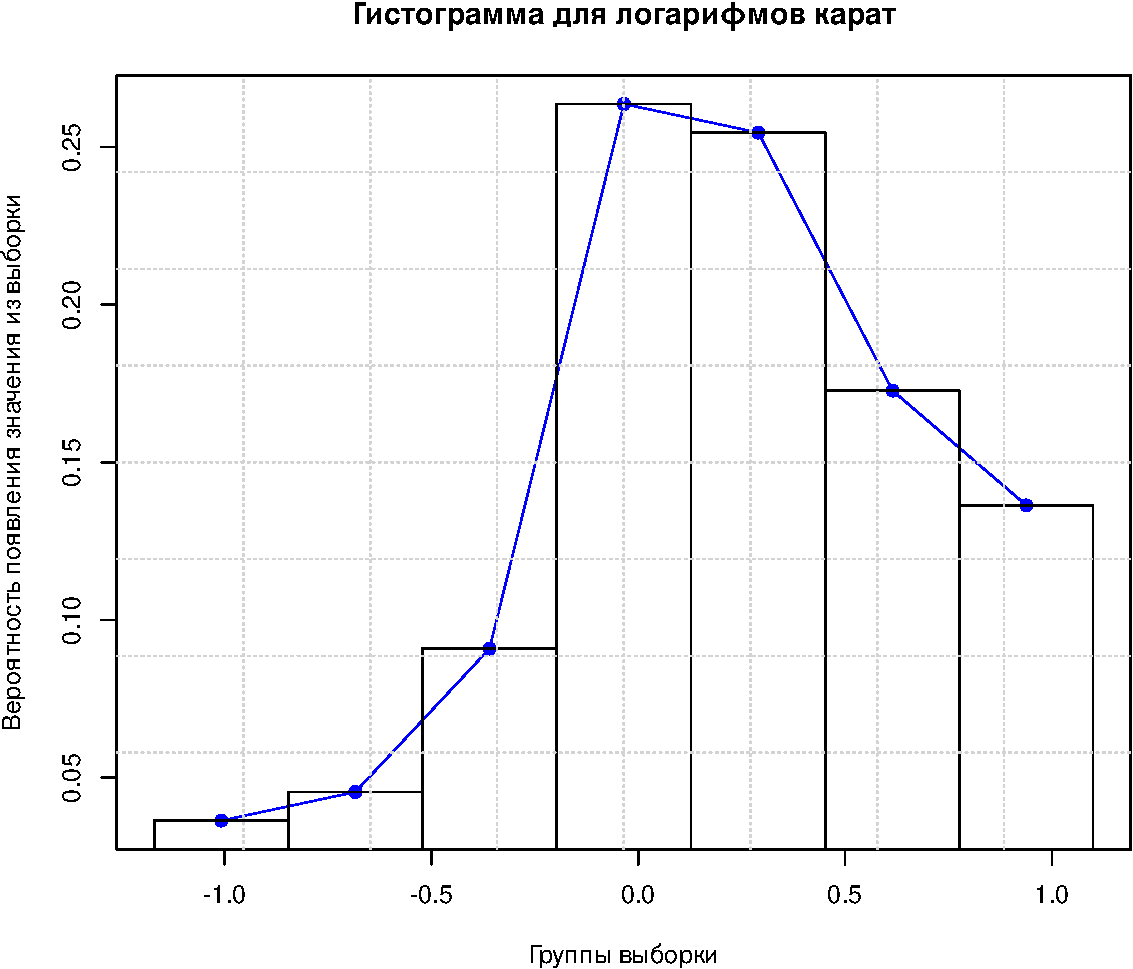
\includegraphics[width=0.6\linewidth]{Prac5_files/figure-latex/unnamed-chunk-6-1} \end{center}

\(\ \)

\begin{verbatim}
##    groupnames abs_freq   rel_freq  low high   med    h
## 1 (5.84,6.41]        3 0.02727273 5.84 6.41 6.125 0.57
## 2 (6.41,6.98]        7 0.06363636 6.41 6.98 6.695 0.57
## 3 (6.98,7.55]        4 0.03636364 6.98 7.55 7.265 0.57
## 4 (7.55,8.11]        8 0.07272727 7.55 8.11 7.830 0.56
## 5 (8.11,8.68]       49 0.44545455 8.11 8.68 8.395 0.57
## 6 (8.68,9.25]       11 0.10000000 8.68 9.25 8.965 0.57
## 7 (9.25,9.82]       28 0.25454545 9.25 9.82 9.535 0.57
\end{verbatim}

\(\ \)

\begin{center}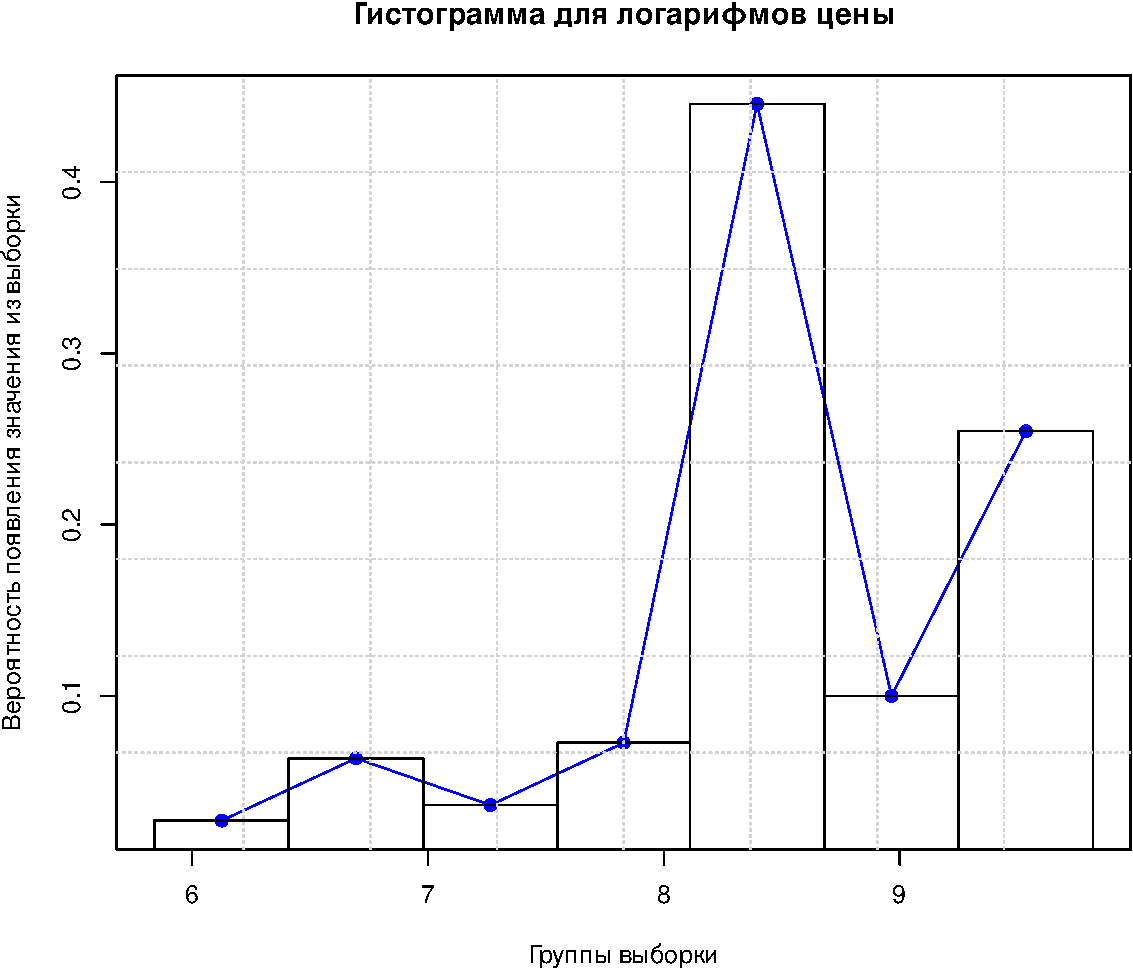
\includegraphics[width=0.6\linewidth]{Prac5_files/figure-latex/unnamed-chunk-8-1} \end{center}

\(\ \)

Для полученных выборок
\(\ X = (x_1, x_2, \dots, x_n), \quad Y = (y_1, y_2, \dots, y_n)\ \)
наши описательные статистики рассчитываем следующим образом:

\[
\overline{x} = \frac{1}{n} \sum \limits_{i=1}^{n} x_i \approx 0.219, \quad \overline{y} = \frac{1}{n} \sum \limits_{i=1}^{n} y_i \approx 8.481
\]

\[
g = 1 + \lfloor log_2(n)\rfloor, \quad  h_x = \frac{max(X) - min(X)}{g}, \quad h_y = \frac{max(Y) - min(Y)}{g},
\]

\[
Z_j = min(X) + j \cdot h_x,\quad L_j = min(Y) + j \cdot h_y, \quad  j=0, 1, \dots, g 
\]

\[
\zeta_i = Z_{i} - Z_{i-1},\quad \theta_i = L_i - L{i-1}, \quad i=1,2,\dots, g,
\]

\[
\sigma_x = \sqrt{\sum\limits_{i = 1}^{g} (\zeta_i - \overline{x})^2 \cdot p^x_i} \approx 0.488, \quad 
\sigma_y = \sqrt{\sum\limits_{i = 1}^{g} (\theta_i - \overline{x})^2 \cdot p^y_i} \approx 0.865
\]

\hypertarget{ux43aux43eux440ux440ux435ux43bux44fux446ux438ux43eux43dux43dux44bux439-ux430ux43dux430ux43bux438ux437-ux447ux438ux441ux43bux43eux432ux44bux445-ux434ux430ux43dux43dux44bux445}{%
\subsection{\texorpdfstring{\textbf{Корреляционный анализ числовых
данных}}{Корреляционный анализ числовых данных}}\label{ux43aux43eux440ux440ux435ux43bux44fux446ux438ux43eux43dux43dux44bux439-ux430ux43dux430ux43bux438ux437-ux447ux438ux441ux43bux43eux432ux44bux445-ux434ux430ux43dux43dux44bux445}}

\hypertarget{ux442ux435ux441ux442-ux433ux435ux442ux435ux440ux43eux441ux43aux435ux434ux430ux441ux442ux438ux447ux43dux43eux441ux442ux438-ux434ux43bux44f-ux440ux44fux434ux430-ux434ux430ux43dux43dux44bux445}{%
\subsection{\texorpdfstring{\textbf{Тест гетероскедастичности для ряда
данных}}{Тест гетероскедастичности для ряда данных}}\label{ux442ux435ux441ux442-ux433ux435ux442ux435ux440ux43eux441ux43aux435ux434ux430ux441ux442ux438ux447ux43dux43eux441ux442ux438-ux434ux43bux44f-ux440ux44fux434ux430-ux434ux430ux43dux43dux44bux445}}

\hypertarget{ux43fux43eux441ux442ux440ux43eux435ux43dux438ux435-ux43bux438ux43dux435ux439ux43dux43eux439-ux43cux43eux434ux435ux43bux438-ux440ux435ux433ux440ux435ux441ux441ux438ux438}{%
\subsection{\texorpdfstring{\textbf{Построение линейной модели
регрессии}}{Построение линейной модели регрессии}}\label{ux43fux43eux441ux442ux440ux43eux435ux43dux438ux435-ux43bux438ux43dux435ux439ux43dux43eux439-ux43cux43eux434ux435ux43bux438-ux440ux435ux433ux440ux435ux441ux441ux438ux438}}

\hypertarget{ux43eux446ux435ux43dux43aux430-ux441ux442ux430ux442ux438ux441ux442ux438ux447ux435ux441ux43aux43eux439-ux437ux43dux430ux447ux438ux43cux43eux441ux442ux438-ux43aux43eux44dux444ux444ux438ux446ux438ux435ux43dux442ux43eux432-ux43bux438ux43dux435ux439ux43dux43eux439-ux43cux43eux434ux435ux43bux438-ux440ux435ux433ux440ux435ux441ux441ux438ux438}{%
\subsection{\texorpdfstring{\textbf{Оценка статистической значимости
коэффициентов линейной модели
регрессии}}{Оценка статистической значимости коэффициентов линейной модели регрессии}}\label{ux43eux446ux435ux43dux43aux430-ux441ux442ux430ux442ux438ux441ux442ux438ux447ux435ux441ux43aux43eux439-ux437ux43dux430ux447ux438ux43cux43eux441ux442ux438-ux43aux43eux44dux444ux444ux438ux446ux438ux435ux43dux442ux43eux432-ux43bux438ux43dux435ux439ux43dux43eux439-ux43cux43eux434ux435ux43bux438-ux440ux435ux433ux440ux435ux441ux441ux438ux438}}

\hypertarget{ux43eux446ux435ux43dux43aux430-ux430ux434ux435ux43aux432ux430ux442ux43dux43eux441ux442ux438-ux43bux438ux43dux435ux439ux43dux43eux439-ux43cux43eux434ux435ux43bux438-ux440ux435ux433ux440ux435ux441ux441ux438ux438}{%
\subsection{\texorpdfstring{\textbf{Оценка адекватности линейной модели
регрессии}}{Оценка адекватности линейной модели регрессии}}\label{ux43eux446ux435ux43dux43aux430-ux430ux434ux435ux43aux432ux430ux442ux43dux43eux441ux442ux438-ux43bux438ux43dux435ux439ux43dux43eux439-ux43cux43eux434ux435ux43bux438-ux440ux435ux433ux440ux435ux441ux441ux438ux438}}

\hypertarget{ux43eux446ux435ux43dux43aux430-ux43fux440ux43eux433ux43dux43eux437ux43dux43eux433ux43e-ux438ux43dux442ux435ux440ux432ux430ux43bux430-ux434ux43bux44f-ux43bux438ux43dux435ux439ux43dux43eux439-ux43cux43eux434ux435ux43bux438-ux440ux435ux433ux440ux435ux441ux441ux438ux438}{%
\subsection{\texorpdfstring{\textbf{Оценка прогнозного интервала для
линейной модели
регрессии}}{Оценка прогнозного интервала для линейной модели регрессии}}\label{ux43eux446ux435ux43dux43aux430-ux43fux440ux43eux433ux43dux43eux437ux43dux43eux433ux43e-ux438ux43dux442ux435ux440ux432ux430ux43bux430-ux434ux43bux44f-ux43bux438ux43dux435ux439ux43dux43eux439-ux43cux43eux434ux435ux43bux438-ux440ux435ux433ux440ux435ux441ux441ux438ux438}}

\hypertarget{ux442ux435ux43cux44b-ux432ux43eux43fux440ux43eux441ux43eux432-ux43dux430-ux437ux430ux449ux438ux442ux443-ux43fux440ux430ux43aux442ux438ux447ux435ux441ux43aux43eux439-ux440ux430ux431ux43eux442ux44b}{%
\section{\texorpdfstring{\textbf{Темы вопросов на защиту практической
работы}}{Темы вопросов на защиту практической работы}}\label{ux442ux435ux43cux44b-ux432ux43eux43fux440ux43eux441ux43eux432-ux43dux430-ux437ux430ux449ux438ux442ux443-ux43fux440ux430ux43aux442ux438ux447ux435ux441ux43aux43eux439-ux440ux430ux431ux43eux442ux44b}}

\begin{enumerate}
\def\labelenumi{\arabic{enumi}.}
\tightlist
\item
  Задачи корреляционного анализа. Выборочный коэффициент линейной
  корреляции (Пирсона) и его свойства. Шкала Чеддока.
\item
  Выборочный коэффициент линейной корреляции (Пирсона) и его свойства.
  Оценка значимости коэффициента корреляции.
\item
  Корреляция и причинная связь. Проблемы корреляционного анализа.
\item
  Ранговая корреляция. Коэффициент ранговой корреляции Спирмена.
\item
  Задачи регрессионного анализа. Функциональная и статистическая связь.
  Аппроксимационные модели. Параметрическое множество функций.
\item
  Линейная регрессия. Определение коэффициентов линейной модели методом
  наименьших квадратов.
\item
  Проверка значимости полученных коэффициентов модели. Проверка
  адекватности модели с помощью критерия Фишера.
\item
  Доверительный интервал прогноза. Проверка адекватности модели с
  помощью критерия Фишера.
\end{enumerate}

\end{document}
